\documentclass[11pt,aspectratio=169]{beamer}

\usepackage{amsmath}
\usepackage{amssymb}
\usepackage{amsfonts}
\usepackage{booktabs}
\usepackage{graphicx}
\usepackage{adjustbox}
\usepackage{comment}
\usepackage{xspace}
\usepackage{appendixnumberbeamer}

\usepackage[
  backend=biber,
  style=authoryear,
  maxcitenames=2,
  mincitenames=1,
  maxbibnames=10,
  minbibnames=1,
  hyperref=false,
  uniquelist=false,
  uniquename=false
]{biblatex}

\let\oldparencite\parencite
\renewcommand{\parencite}[2][]{%
  \footnotesize {\tiny \oldparencite[#1]{#2}} \normalsize%
}
\renewcommand*{\bibfont}{\scriptsize}
\addbibresource{../../july_draft/causal_effect_schools.bib}
\AtEveryBibitem{%
  \clearfield{url}%
  \clearfield{urldate}%
  \clearfield{urlyear}%
  \clearfield{urlmonth}%
  \clearfield{urlday}%
  \clearfield{doi}%
  \clearfield{issn}%
  \clearfield{isbn}%
  \clearfield{eprint}%
  \clearfield{language}%
  \clearlist{language}%
}
\DeclareBibliographyCategory{schoolquality}
\DeclareBibliographyCategory{collegechoice}
\DeclareBibliographyCategory{assignmentmethods}
\addtocategory{schoolquality}{jackson_what_2018,beuermann_what_2023,rose_effects_2022,kirkeboen_field_2016}
\addtocategory{collegechoice}{hoxby_what_2015,dynarski_closing_2021,hastings_informed_2016,chetty_diversifying_2025}
\addtocategory{assignmentmethods}{abdulkadiroglu_research_2017,angrist_leveraging_2017,walters_chapter_2024,chetty_measuring_2014-1}

\usetheme[progressbar=frametitle]{metropolis}
\metroset{sectionpage=none}
\setbeamercolor{alerted text}{fg=mDarkTeal}

\newcommand{\key}[1]{\textcolor{mDarkTeal}{\textbf{#1}}}
\setbeamercolor{sampleneutral}{fg=black,bg=black!6}
\setbeamercolor{samplemain}{fg=black,bg=mDarkTeal!24}
\setbeamercolor{samplescore}{fg=white,bg=mDarkTeal}
\newcommand{\samplestep}[3]{%
  \begin{beamercolorbox}[wd=\linewidth,sep=0.30em,rounded=true]{#1}
    \begin{minipage}[c]{0.68\linewidth}
      \raggedright\footnotesize #2
    \end{minipage}\hfill
    \begin{minipage}[c]{0.27\linewidth}
      \raggedleft\large\bfseries #3
    \end{minipage}
  \end{beamercolorbox}%
}
\newcommand{\samplearrow}{\par\vspace{0.01em}{\color{mDarkTeal}\scriptsize$\blacktriangledown$}\par\vspace{0.01em}}

\newenvironment{wideitemize}{%
  \begin{minipage}{0.92\textwidth}
  \begin{itemize}
  \addtolength{\itemsep}{0.75em}
}{%
  \end{itemize}
  \end{minipage}
}

\title{Do High Schools Shape College Choices?}
\subtitle{Evidence from Centralized Assignment in Chile}
\author{Bruno E. Aravena-Mag\"uida}
\institute{University of Chicago}
\date{August 2026}

\begin{document}

% 1
\begin{frame}[plain,t]
\vspace{1.25cm}
{\LARGE\bfseries Do High Schools Shape College Choices?\par}
\vspace{-0.05em}
{\large Evidence from Centralized Assignment in Chile\par}
\vspace{0.8em}
\rule{\textwidth}{0.4pt}
\vspace{0.9em}

Bruno E. Aravena-Mag\"uida\\
University of Chicago

\vspace{0.6em}
August 2026
\end{frame}

\section{Question}

% 2
\begin{frame}{High schools may shape choices that test-score measures miss}

  We know that:\par
  \vspace{0.05em}
  \begin{wideitemize}
  \addtolength{\itemsep}{-0.55em}
  \item Despite school quality being usually summarized by test scores, ample evidence of multiple dimensions. \parencite{jackson_what_2018,beuermann_what_2023,rose_effects_2022}

  \item College application and enrollment differ across groups even conditional on achievement, ample room for interventions. \parencite{hoxby_what_2015,dynarski_closing_2021,hastings_informed_2016,chetty_diversifying_2025}

  \item Returns differ substantially across institutions and especially across fields. \parencite{kirkeboen_field_2016}
\end{wideitemize}

\begin{alertblock}{Research Question}
\vspace{0.35em}
Do high schools causally shape college choices, and are those effects captured by achievement value added?
\end{alertblock}
\end{frame}

\begin{frame}[plain]
\centering
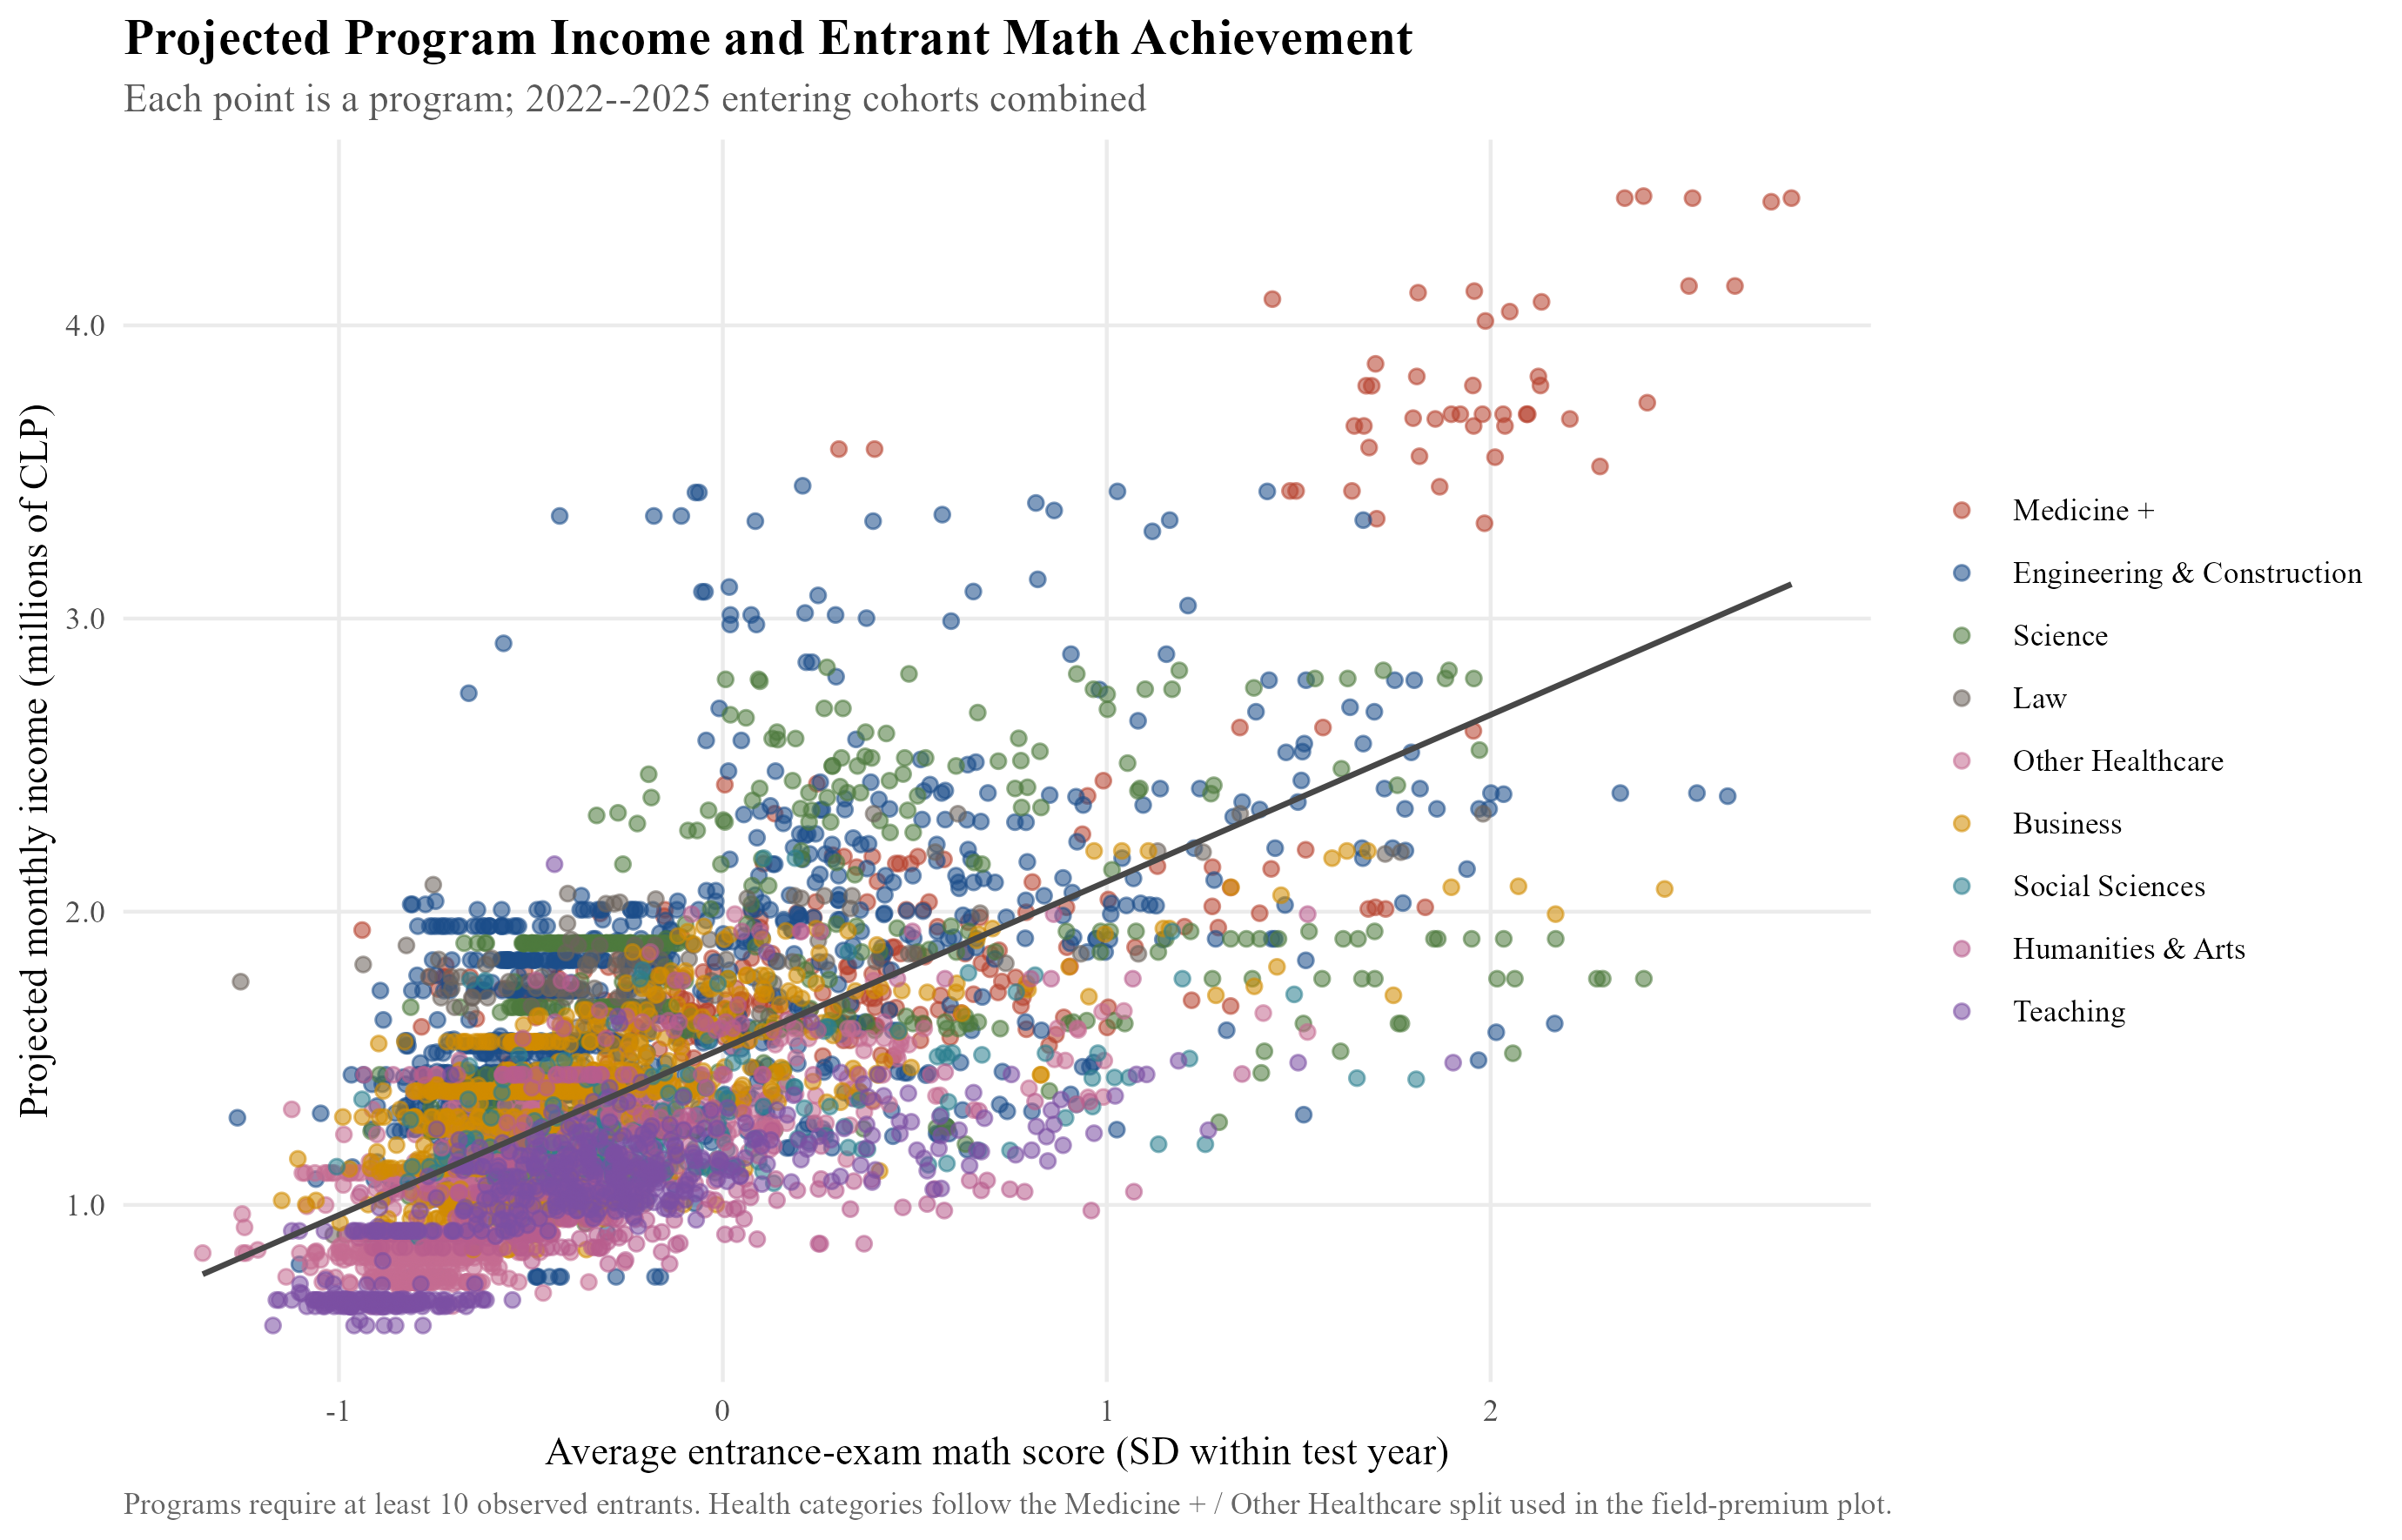
\includegraphics[height=0.98\paperheight,keepaspectratio]{../../../output/figures/mifuturo_matricula_income/program_income_vs_entering_math_by_field.png}
\end{frame}

% 3
\begin{frame}{This paper}
\small

  \begin{itemize}
  \item I combine centralized high school assignment (with random tie-breaking) with information about higher educational choices.
  \item For each outcome I proceed in two steps: 
\end{itemize}
\vspace{0.35em}

\begin{columns}[T,onlytextwidth]
  \column{0.46\textwidth}
  \textbf{1. Broad national panel}

  Estimate outcome-specific school value added using rich pre-treatment controls. 
  Apply Empirical Bayes to reduce noise in estimates. \parencite{chetty_measuring_2014-1,walters_chapter_2024}.

  \vspace{0.05em}
  \centering
  $\widehat V_j^{m,EB}$

  \column{0.46\textwidth}
  \textbf{2. SAE lottery sample}

  Test whether an offer to a higher-value-added school (gains in   $\widehat V_j^{m,EB}$) causally improves the same outcome.

  \vspace{0.4em}
  \centering
  $\varphi^m$
\end{columns}

\end{frame}



\begin{frame}{Preview of Results}
\centering
\scriptsize
\setlength{\tabcolsep}{5pt}
\renewcommand{\arraystretch}{1.35}
\begin{tabular}{lcccc}
\toprule
Outcome
& \shortstack{Outcome\\mean}
& \shortstack{$P_{90}-P_{10}$\\VA difference}
& $\varphi$
& \shortstack{Implied causal gain\\$(P_{90}-P_{10})\times\varphi$} \\
\midrule
Math & 0.043 & 0.492 SD & 0.884 & \textbf{0.435 SD} \\
%Verbal & 0.049 & 0.374 SD & 0.885 & \textbf{0.331 SD} \\
%High-premium institution & 0.142 & 23.4 pp & 0.497 & \textbf{11.6 pp} \\
High-premium field & 0.347 & 12.3 pp & 0.803 & \textbf{9.9 pp} \\
%Log projected income & 13.893 & 0.183 log points & 0.311 & \textbf{0.057 log points} \\
\bottomrule
\end{tabular}

\vspace{0.9em}
\footnotesize
 The final column is the lottery-validated causal gain implied by moving from a $P_{10}$ to a $P_{90}$ value-added school.
\end{frame}

\section{Data and Context}

% 5
\begin{frame}{Five outcomes capture achievement and the college option entered}
\begin{columns}[T,onlytextwidth]
  \column{0.45\textwidth}
  \textbf{Achievement in higher-education exams}
  \begin{itemize}
    \item standardized math score;
    \item standardized verbal score.
  \end{itemize}

  \column{0.51\textwidth}
  \textbf{Higher-education choices}
  \begin{itemize}
    \addtolength{\itemsep}{0.5em}
    \item \textbf{log projected income}, based on MiFuturo (avg. wage per program-institution reported by govt.) 
    \item enrollment in a \textbf{high-premium field} (binary);
    \item enrollment in a \textbf{high-premium institution} (binary);
  \end{itemize}
\end{columns}

\vspace{1em}
\begin{alertblock}{Outcome convention}
Non-enrollment is coded as zero for the premium indicators and enters projected income at a minimum-wage proxy.
\end{alertblock}
\end{frame}

\begin{frame}{Projected-income premia vary sharply across fields}
\centering
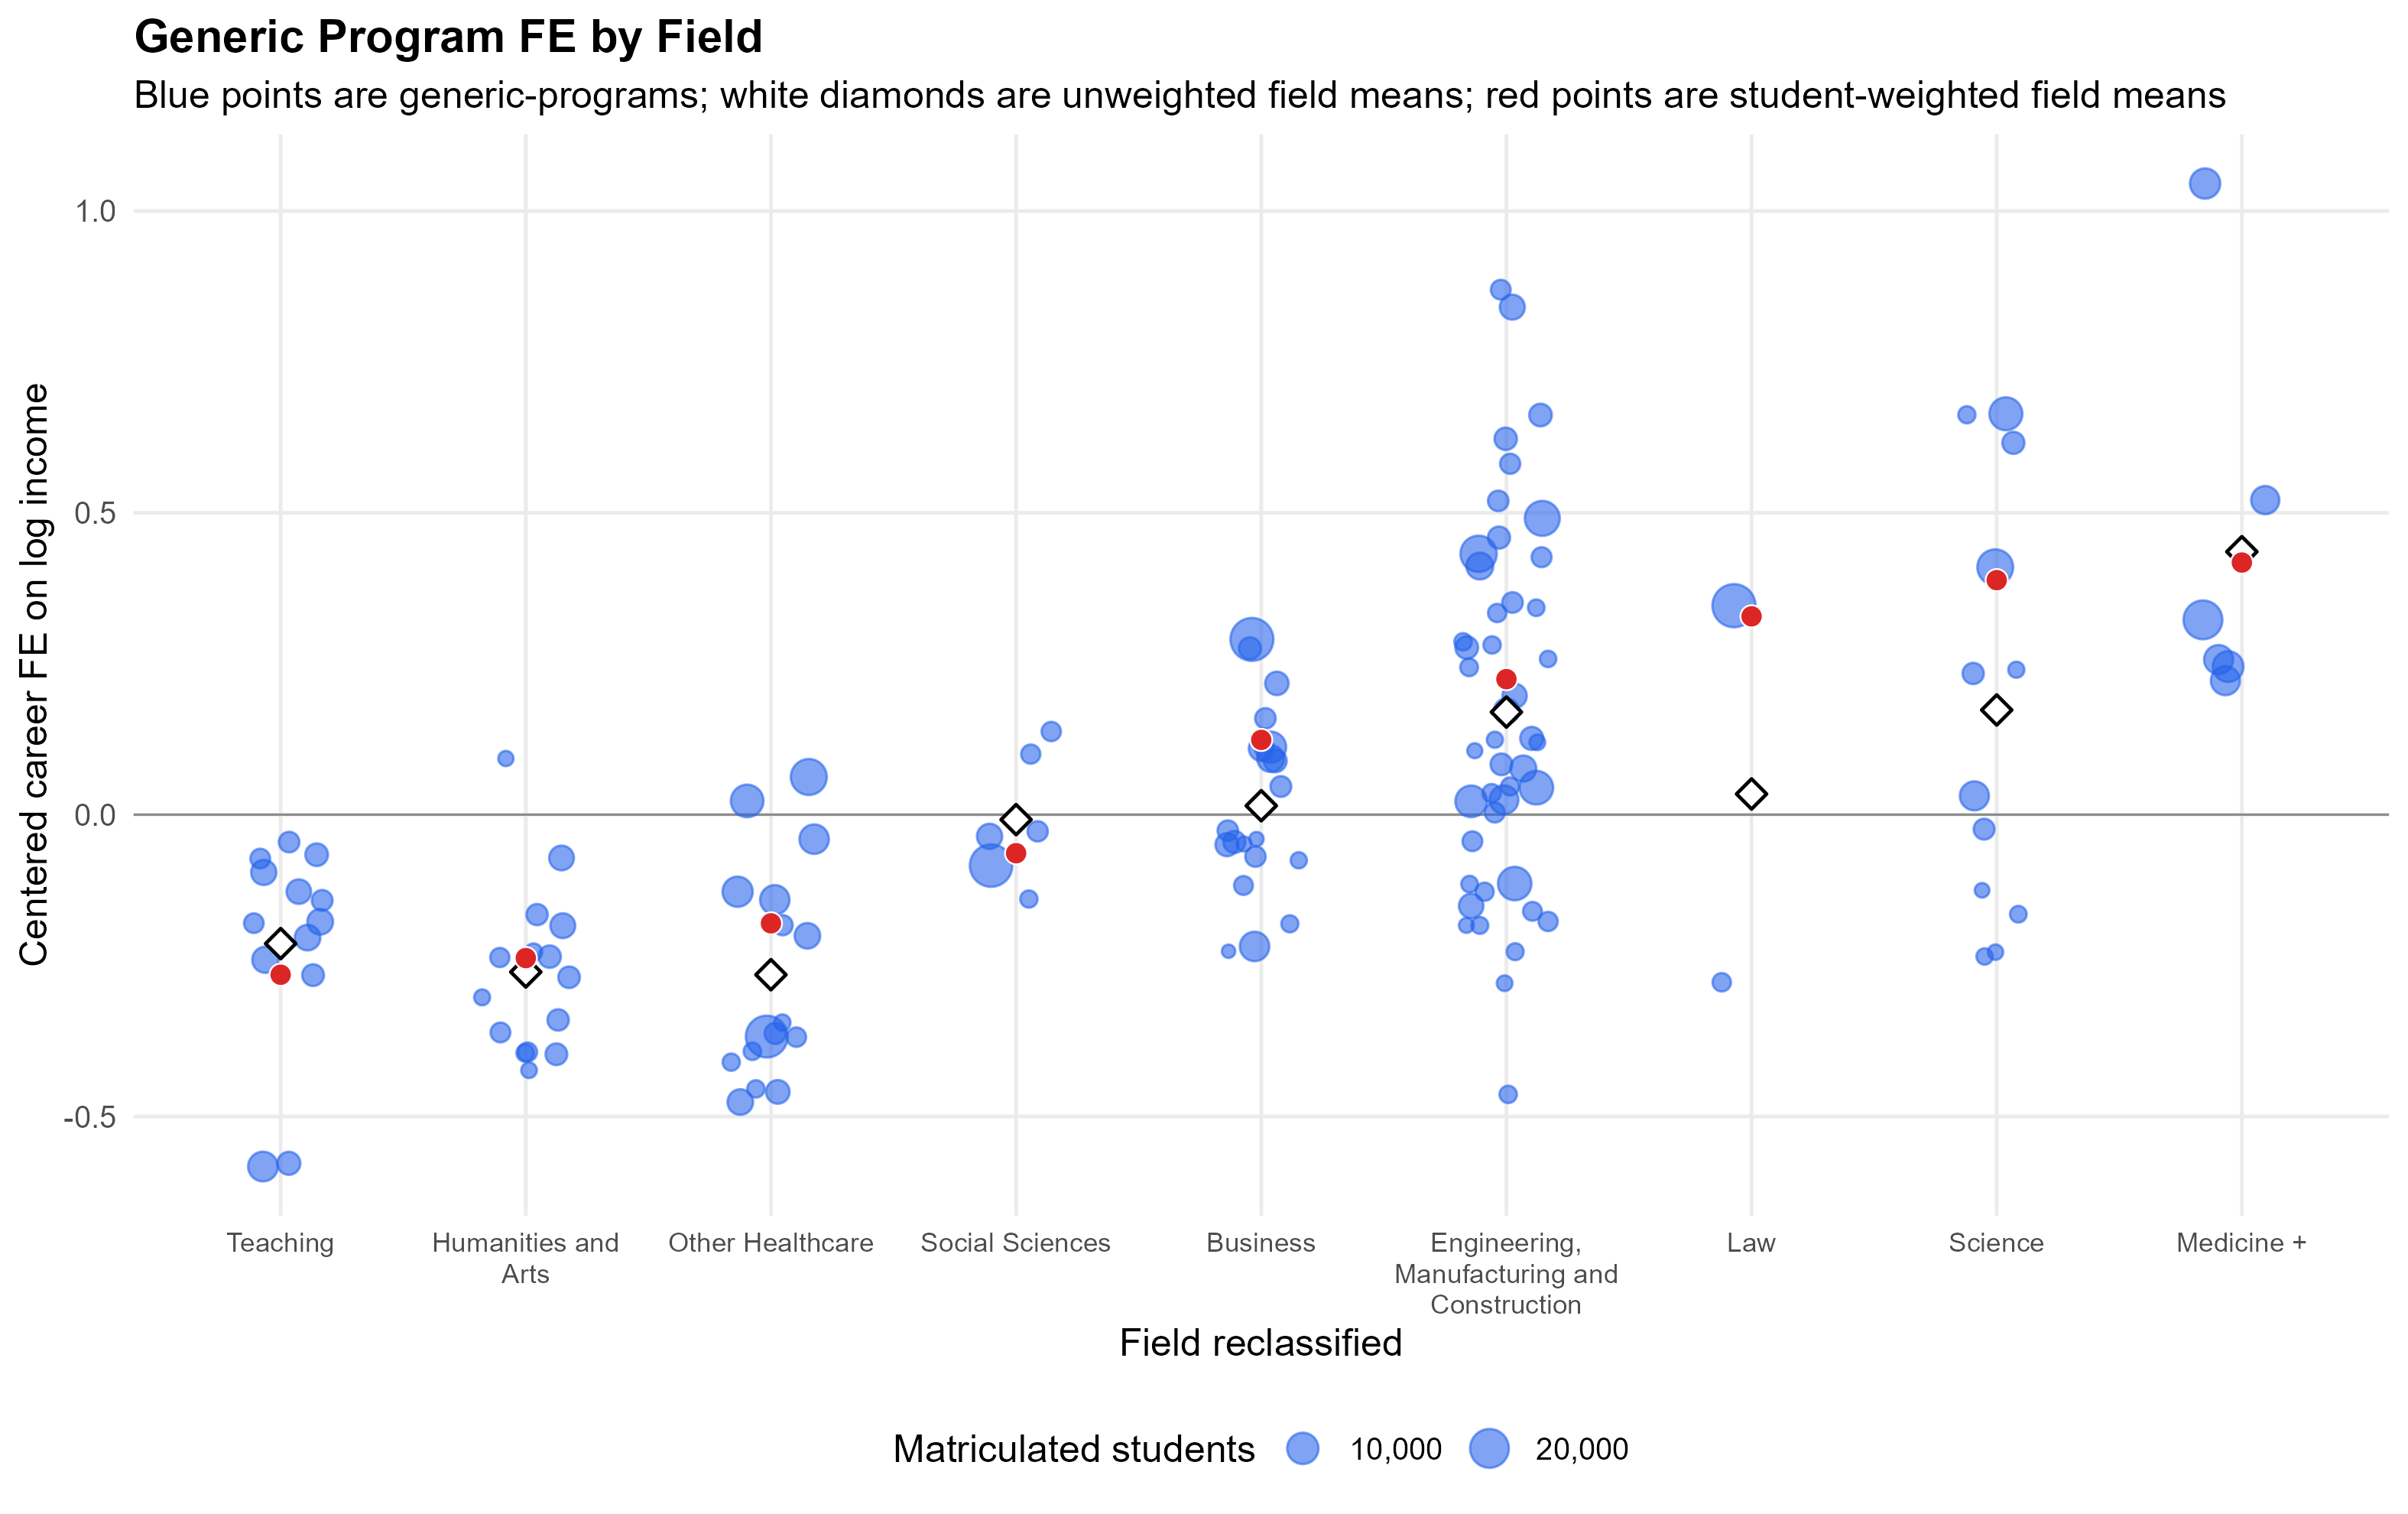
\includegraphics[width=0.92\linewidth,height=0.72\textheight,keepaspectratio]{../../../output/figures/mifuturo_matricula_income/area_carrera_generica_program_fe_by_field.png}

\vspace{-0.2em}
\footnotesize
The high-premium-field outcome includes Science, Law, Engineering/Manufacturing/Construction, and Medicine+.
\end{frame}

\begin{frame}{Centralized high-school assignment in Chile}
\small
\begin{wideitemize}
  \addtolength{\itemsep}{-0.2em}
  \item The \textit{Sistema de Admisi\'on Escolar} (SAE) began regionally in 2017 and became national in 2018. It covers public and private-subsidized schools, which enroll about 91\% of students.
  \item Families applying to grade 9 submit ranked school lists. Student-proposing Deferred Acceptance combines rankings, vacancies, and priorities, using random tie-breakers within oversubscribed priority groups.
  \item I replicate the assignment algorithm and recover each applicant's school-offer probabilities through repeated counterfactual lottery draws.
\end{wideitemize}

\vspace{0.15em}
\begin{alertblock}{Replication check}
\footnotesize
Using the original lottery numbers, the replicated mechanism reproduces more than 99\% of observed first-round assignments in every 2018--2021 cohort.
\end{alertblock}
\end{frame}


% 4
\begin{frame}{Sample description}
\centering
\begin{columns}[T,onlytextwidth]
  \column{0.455\textwidth}
  \centering
  {\large\bfseries Value-added estimation}\par
  \vspace{0.18em}

  \samplestep{sampleneutral}{Grade-8 universe, 2017--2020}{944,510}
  \samplearrow
  \samplestep{samplescore}{Complete value-added controls\\[-0.15em]
    \scriptsize Choice + income VA base}{757,999}
  \samplearrow
  \samplestep{samplescore}{Math or verbal score observed\\[-0.15em]
    \scriptsize Math + verbal VA}{571,110}

  \column{0.455\textwidth}
  \centering
  {\large\bfseries Lottery IV}\par
  \vspace{0.18em}

  \samplestep{sampleneutral}{Timely grade-9 SAE applicants, 2018--2021}{409,737}
  \samplearrow
  \samplestep{sampleneutral}{Applicants with assignment risk}{226,195}
  \samplearrow
  \samplestep{sampleneutral}{Complete grade-4 SIMCE controls}{139,317}
  \samplearrow
  \samplestep{samplescore}{Exam takers with math or verbal score\\[-0.15em]
    \scriptsize All five IV outcomes}{95,705}
\end{columns}
\end{frame}

\section{Methodology}


\begin{frame}{Step 1: Value Added Estimation}
\small
\[
Y_i^m
=
\alpha^m
+\lambda_{s(i)}^m
+X_i'\Gamma^m
+\mu_i^m,
\qquad
\widehat V_j^m=\widehat\lambda_j^m-\overline{\widehat\lambda}^{\,m}_{w}.
\]

\begin{wideitemize}
  \item Estimate a separate school fixed effect per each outcome with universe.
  \item $X_i$ includes grade-4 (national) achievement polynomials, family background, middle-school fixed-effect plus grades and attendance, cohort, gender, age, and home location.
  \item These measures remain observational: sorting not absorbed by $X_i$ can contaminate $\widehat V_j^m$.
  \item  $\widehat V_j^m$ are demeaned so average value-added estimate is zero. 
\end{wideitemize}
\end{frame}

\begin{frame}{Step 1.2: Empirical Bayes shrinks less precise school estimates more strongly}
\small
\[
\widehat\tau_m^2
=
\max\left\{
\operatorname{Var}_{\omega}(\widehat V_j^m)
-\sum_j\omega_j(se_j^m)^2,
0
\right\},
\quad
\lambda_j^m
=
\frac{\widehat\tau_m^2}{\widehat\tau_m^2+(se_j^m)^2},
\quad
\widehat V_j^{m,EB}=\lambda_j^m\widehat V_j^m.
\]

\begin{wideitemize}
  \item Large, precisely estimated schools remain close to their original fixed effects.
  \item Small or noisy schools move toward the student-weighted mean of zero. \parencite{walters_chapter_2024}
  \item Shrinkage improves the signal-to-noise ratio; it does not create a separate causal estimator.
\end{wideitemize}
\end{frame}


\begin{frame}{Lottery identification: selection and randomization}
\footnotesize
\begin{columns}[T,onlytextwidth]
  \column{0.48\textwidth}
  \textbf{Ranked lists capture selection}
  \begin{itemize}
    \item Challenge of studying causal effects of schools is selection.
    \item Families reveal their `types' through their ranked school lists.
    \item Rankings (and priorities) imply each applicant's assignment probabilities $p_i$.
    \item $E_i^{m,EB}=\sum_j p_{ij}\widehat V_j^{m,EB}$ summarizes the school value added expected from the choices of that student `type'.
  \end{itemize}

  \column{0.48\textwidth}
  \textbf{Tie-breakers generate exogenous variation}
  \begin{itemize}
    \item SAE sees only ranked lists and generates random tie-breakers.
    \item It does not see prior achievement, family background, potential outcomes, etc.
    \item Conditional on $p_i$, the tie-breaker makes the school offered quasi-random.
  \end{itemize}
\end{columns}

%\vspace{0.15em}
%\begin{alertblock}{Identification}
%\centering
%\textbf{Control for selection:}\quad
%rankings and priorities $\longrightarrow p_i \longrightarrow E_i^{m,EB}$\\[0.3em]
%\textbf{Instrument:}\quad
%random tie-breaker $\longrightarrow O_i^{m,EB}-E_i^{m,EB}
% \longrightarrow A_i^{m,EB}\longrightarrow Y_i^m$

%\vspace{0.2em}
%\scriptsize The first stage asks whether the offer changes attended-school value added; the second stage estimates its effect on the outcome. \parencite{abdulkadiroglu_research_2017}
%\end{alertblock}
\end{frame}


\begin{frame}{First Stage: Lottery offers shift attended-school value added}
\small
\[
A_i^{m,EB}
=
a^m
+\kappa^m O_i^{m,EB}
+\rho_A^m E_i^{m,EB}
+W_i'\delta_A^m
+\nu_i^m.
\]

\begin{columns}[T,onlytextwidth]
  \column{0.47\textwidth}
  \textbf{Instrument and treatment}
  \begin{itemize}
    \item $O_i^{m,EB}=\widehat V_{Z_i}^{m,EB}$: value added of the first-round offered school.
    \item $A_i^{m,EB}=\widehat V_{D_i}^{m,EB}$: value added of the school ultimately attended.
  \end{itemize}

  \column{0.47\textwidth}
  \textbf{Conditioning on assignment risk}
  \begin{itemize}
    \item $E_i^{m,EB}=\sum_j p_{ij}\widehat V_j^{m,EB}$ summarizes the applicant's simulated offer probabilities.
    \item Conditional on $p_i$, random tie-breakers generate quasi-experimental variation in $O_i^{m,EB}$.
    \item $W_i$: cohort indicators, gender, age, and grade-4 SIMCE math and language scores.
  \end{itemize}
\end{columns}

%\vspace{0.25em}
%\footnotesize
%The first stage asks whether an offer from a higher-value-added school induces attendance at a higher-value-added school. \parencite{abdulkadiroglu_research_2017}
\end{frame}
% 6
\begin{frame}{Second Stage: Estimate pass-through using the lottery}
\small
\[
Y_i^m
=
\alpha^m
+\varphi^m A_i^{m,EB}
+\rho^m E_i^{m,EB}
+W_i'\delta^m
+\eta_i^m,
\qquad
A_i^{m,EB}\ \text{instrumented by}\ O_i^{m,EB}.
\]

\begin{wideitemize}
  \addtolength{\itemsep}{-0.15em}
  \item $Y_i^m$ is the student outcome used to construct value added for outcome $m$.
  \item $E_i^{m,EB}$ absorbs expected value added from the student's assignment portfolio.
  \item $W_i$: cohort indicators, gender, age, and grade-4 SIMCE math and language scores.
  \item $\varphi^m$ measures how much of a lottery-induced increase in attended-school value added passes through into a causal gain in outcome $m$.
\end{wideitemize}

\vspace{0.1em}
\begin{alertblock}{Interpretation}
$\varphi^m=1$: one-for-one pass-through.\hfill
$\varphi^m=0$: no causal content at the lottery margin.
\end{alertblock}
\end{frame}

\section{Results}


% 7
\begin{frame}[label=results_one]{Results: Value added predicts causal gains in all five outcomes}
\centering
\scriptsize
\setlength{\tabcolsep}{6pt}
\begin{tabular}{lccccc}
\toprule
& \multicolumn{2}{c}{Achievement} & \multicolumn{3}{c}{Higher-education choices} \\
\cmidrule(lr){2-3}\cmidrule(lr){4-6}
& Math & Verbal & High-premium inst. & High-premium field & Log proj. income \\
\midrule
$\varphi^{EB}$
& \textbf{0.884***}
& \textbf{0.885***}
& \textbf{0.497***}
& \textbf{0.803***}
& \textbf{0.311***} \\
& (0.073) & (0.087) & (0.111) & (0.100) & (0.103) \\
$N$ & 93,438 & 95,107 & 95,651 & 90,338 & 95,651 \\
\bottomrule
\end{tabular}

\vspace{0.7em}
\begin{wideitemize}
  \item Achievement pass-through is close to one despite the absence of immediately lagged test scores.
  \item School value added also predicts movement into higher-premium institutions, fields, and programs with higher projected income.
\end{wideitemize}

\vspace{0.25em}
\hyperlink{heterogeneity_baseline}{\beamergotobutton{Heterogeneity by baseline achievement}}
\hspace{0.7em}
\hyperlink{heterogeneity_gender}{\beamergotobutton{Heterogeneity by gender}}

\vspace{0.35em}
\tiny Robust standard errors in parentheses. All models control for expected EB value added and baseline covariates. $^{***}p<0.01$.
\end{frame}

% 8
\begin{frame}{Results: Estimates imply economically meaningful 90--10 school differences}
\centering
\scriptsize
\setlength{\tabcolsep}{5pt}
\renewcommand{\arraystretch}{1.35}
\begin{tabular}{lcccc}
\toprule
Outcome
& \shortstack{Outcome\\mean}
& \shortstack{$P_{90}-P_{10}$\\VA difference}
& $\varphi$
& \shortstack{Implied causal gain\\$(P_{90}-P_{10})\times\varphi$} \\
\midrule
Math & 0.043 & 0.492 SD & 0.884 & \textbf{0.435 SD} \\
Verbal & 0.049 & 0.374 SD & 0.885 & \textbf{0.331 SD} \\
High-premium institution & 0.142 & 23.4 pp & 0.497 & \textbf{11.6 pp} \\
High-premium field & 0.347 & 12.3 pp & 0.803 & \textbf{9.9 pp} \\
Log projected income & 13.893 & 0.183 log points & 0.311 & \textbf{0.057 log points} \\
\bottomrule
\end{tabular}

\vspace{0.9em}
\footnotesize
The final column is the lottery-validated causal gain implied by moving from a $P_{10}$ to a $P_{90}$ value-added school.



%\vspace{1em}
%\begin{alertblock}{Interpretation}
%Along the SAE lottery margin, moving across the school value-added distribution changes achievement and the institution, field, and projected earnings of the program students enter.
%\end{alertblock}
\end{frame}

% 9
\begin{frame}[label=cross_outcome_results]{Cross-outcome results: Math and field VA capture different margins}
\centering
\scriptsize
\begin{tabular}{lcccc}
\toprule
& \multicolumn{2}{c}{Math score} & \multicolumn{2}{c}{High-premium field} \\
\cmidrule(lr){2-3}\cmidrule(lr){4-5}
School value-added index & Estimate & SE & Estimate & SE \\
\midrule
Math VA & 0.884*** & (0.073) & -0.184*** & (0.054) \\
High-premium-field VA & 0.099 & (0.126) & 0.803*** & (0.100) \\
\bottomrule
\end{tabular}


\vspace{0.45em}
\tiny
Each cell is a separate lottery IV. The attended-school VA in that row is instrumented by the corresponding offered-school VA; models control for its expected VA and baseline covariates.

\vspace{0.7em}
\begin{columns}[T,onlytextwidth]
  \column{0.47\textwidth}
  \centering
  \textbf{Math VA $\rightarrow$ field choice}

  \vspace{0.25em}
  \normalsize
  $P_{90}-P_{10}$ effect: \key{$-9.1$ pp}

  \footnotesize
  Higher math VA does not proxy for movement into high-premium fields.

  \column{0.47\textwidth}
  \centering
  \textbf{Field VA $\rightarrow$ math score}

  \vspace{0.25em}
  \normalsize
  $P_{90}-P_{10}$ effect: \key{$+0.012$ SD}

  \footnotesize
  The estimate is small and statistically insignificant ($p=0.429$).
\end{columns}

\vspace{0.45em}
\hyperlink{cross_outcome_spec}{\beamergotobutton{Cross-outcome IV specification}}
\end{frame}

\section{Conclusion}

% 10
\begin{frame}{Schools affect higher educational paths through multiple channels}
\begin{wideitemize}
  \item Observational value added predicts lottery-induced causal gains in achievement and the characteristics of higher educational choices.

  \item In the same way we can identify schools with large causal effects in mathematics achievement, we can identify schools that nudge students into high-premium fields and institutions.

  \item The effects are large enough to be relevant. 

  \item Cross-outcome tests suggest that the effects on choices are not predicted by achievement: the effects operate through different margins.
\end{wideitemize}

%\begin{alertblock}{Takeaway}
%High schools shape not only how much students learn, but also the options they perceive and choose.
%\end{alertblock}
\end{frame}

\begin{frame}[standout]
Thanks!

\vspace{0.8em}
\normalsize
brunem@uchicago.edu
\end{frame}

\begin{frame}{School quality references}
\printbibliography[heading=none,category=schoolquality]
\end{frame}

\begin{frame}{College choice references}
\printbibliography[heading=none,category=collegechoice]
\end{frame}

\begin{frame}{Methods references}
\printbibliography[heading=none,category=assignmentmethods]
\end{frame}



%\begin{comment}

\appendix
\section{Extra slides}

\begin{frame}[label=heterogeneity_baseline]{Math pass-through is weakest for students with low baseline achievement}
\begin{columns}[c,onlytextwidth]
  \column{0.62\textwidth}
  \centering
  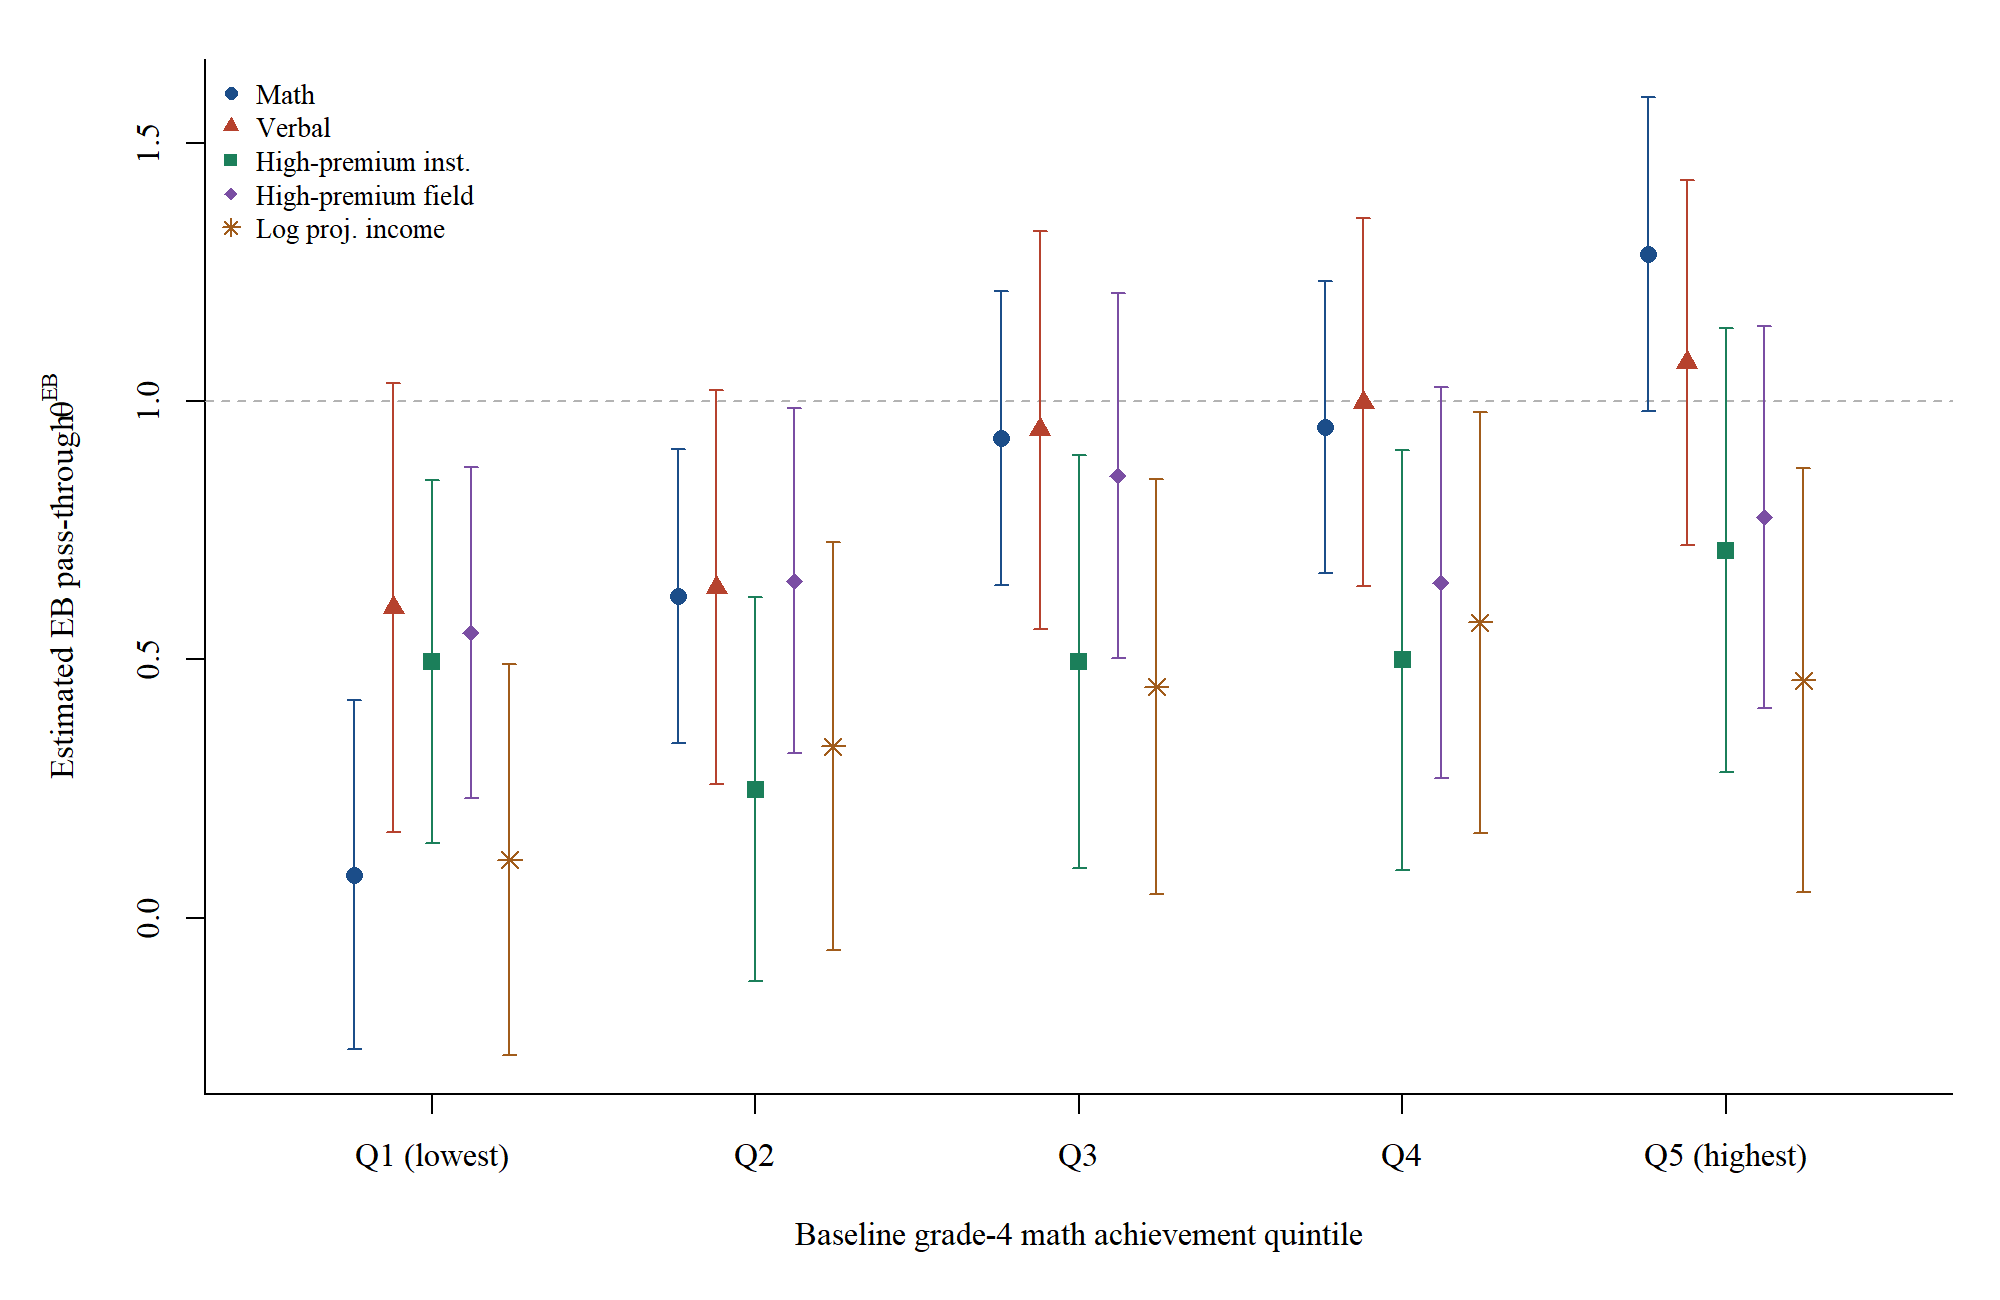
\includegraphics[width=\textwidth]{../../../output/figures/results_section/simce4_math_quintile_primary_five_eb.png}

  \column{0.34\textwidth}
  \begin{itemize}
    \addtolength{\itemsep}{0.6em}
    \item Math: $\widehat\varphi_{Q1}=0.083$ versus $\widehat\varphi_{Q3}=0.929$.
    \item Difference: $-0.846$ ($p<0.01$).
    \item Higher-education pass-through is stable across baseline math quintiles.
  \end{itemize}
\end{columns}
\vspace{0.1em}
\hfill\hyperlink{results_one}{\beamerreturnbutton{Results 1}}
\end{frame}

\begin{frame}[label=heterogeneity_gender]{Achievement value added is more predictive for girls}
\begin{columns}[c,onlytextwidth]
  \column{0.67\textwidth}
  \centering
  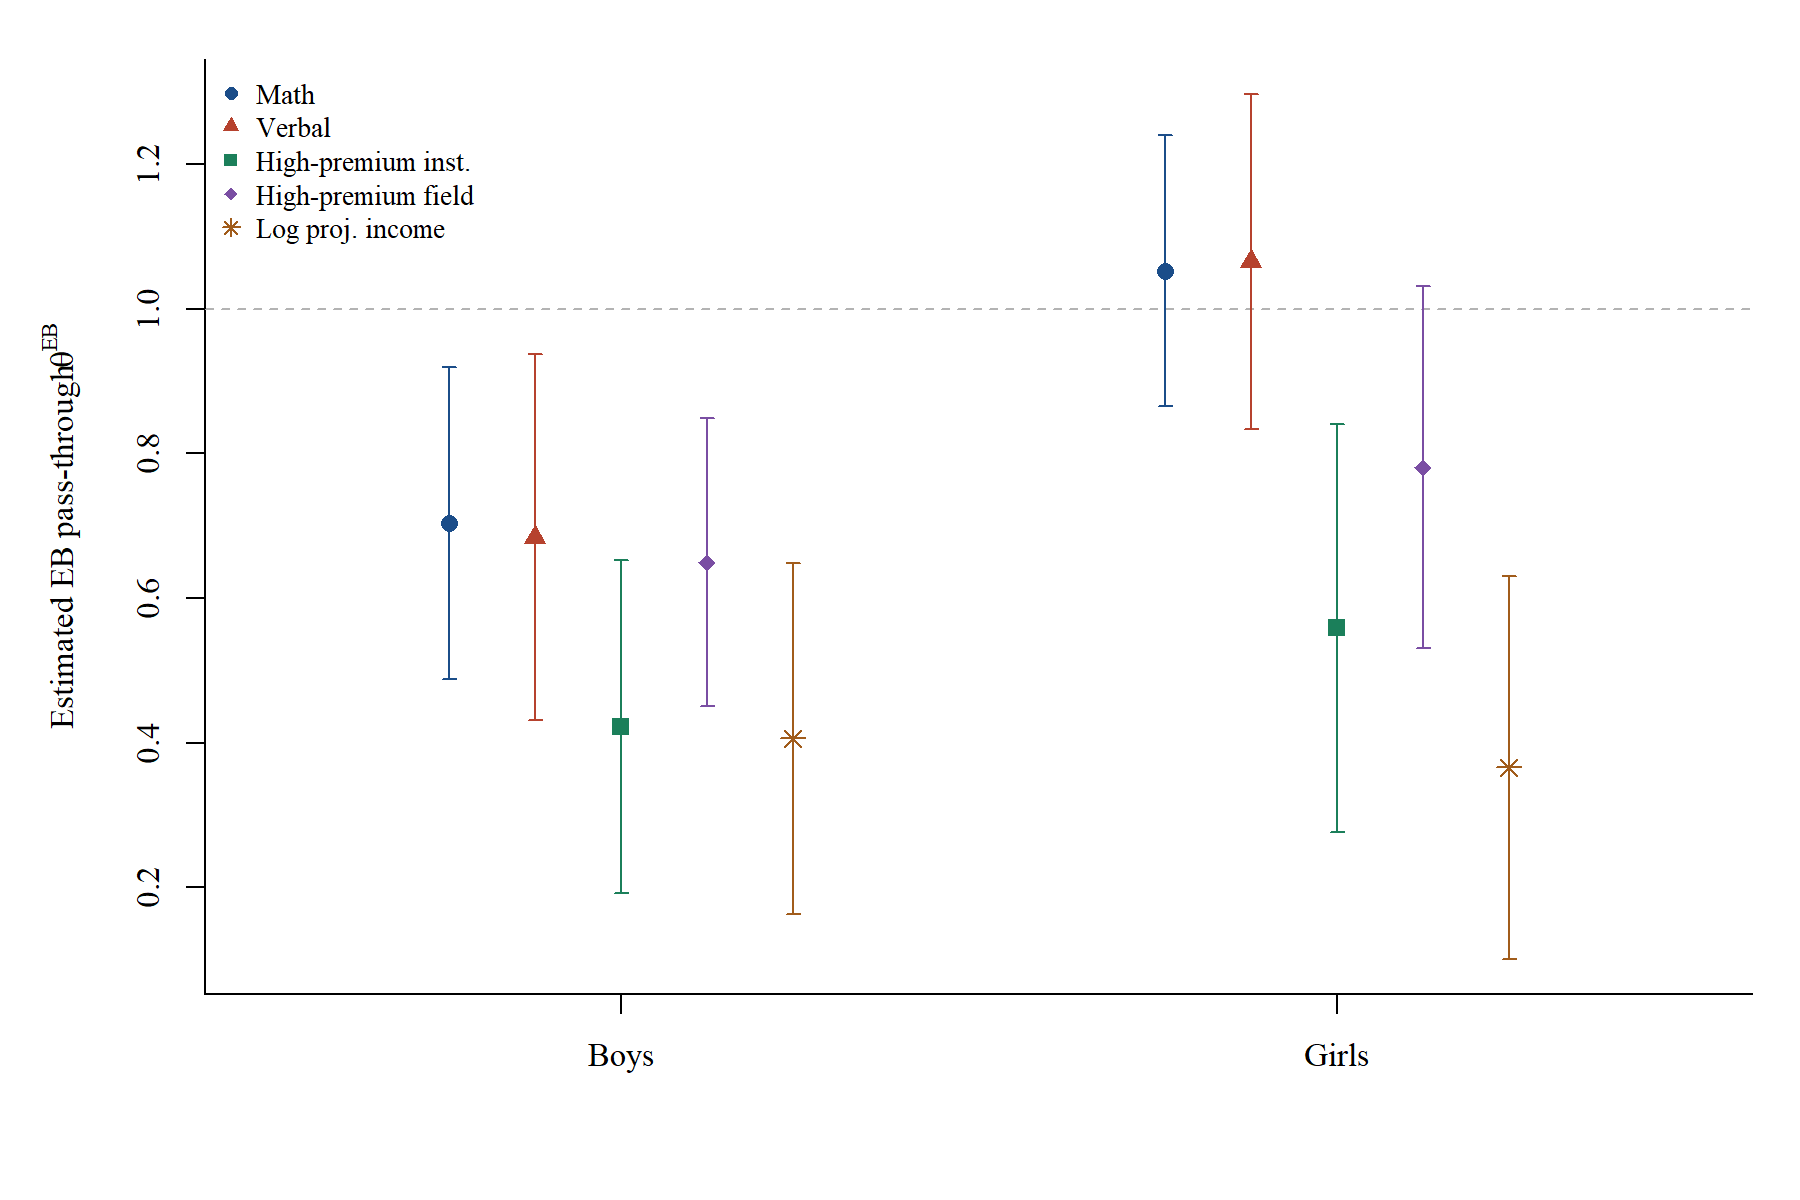
\includegraphics[width=\textwidth]{../../../output/figures/results_section/primary_five_eb_by_gender.png}

  \column{0.29\textwidth}
  \small
  \begin{itemize}
    \addtolength{\itemsep}{0.4em}
    \item Math: girls' pass-through is 0.349 higher ($p=0.017$).
    \item Verbal: girls' pass-through is 0.382 higher ($p=0.029$).
    \item Gender differences are small and insignificant for the choice outcomes.
  \end{itemize}
\end{columns}
\vspace{0.1em}
\hfill\hyperlink{results_one}{\beamerreturnbutton{Results 1}}
\end{frame}

\begin{comment}

\begin{frame}[label=cross_outcome_spec]{IV specification}
\small
\[
\begin{aligned}
Y_i^{F}
&=
\alpha_F
+\psi_{F\leftarrow M}A_i^{M,EB}
+\rho_F E_i^{M,EB}
+W_i'\delta_F
+\eta_i^F, \\
Y_i^{M}
&=
\alpha_M
+\psi_{M\leftarrow F}A_i^{F,EB}
+\rho_M E_i^{F,EB}
+W_i'\delta_M
+\eta_i^M.
\end{aligned}
\]

\begin{wideitemize}
  \addtolength{\itemsep}{-0.1em}
  \item In the first equation, math VA of the attended school is instrumented with math VA of the offered school.
  \item In the second, high-premium-field VA of the attended school is instrumented with field VA of the offered school.
  \item $E_i^{M,EB}$ and $E_i^{F,EB}$ are the corresponding assignment-portfolio risk controls.
  \item The equations are estimated separately: no residualization or ordered decomposition is used.
\end{wideitemize}

\vspace{0.2em}
\hfill\hyperlink{cross_outcome_results}{\beamerreturnbutton{Cross-outcome results}}
\end{frame}


\begin{frame}{Chile's centralized assignment system creates national lottery variation}
\begin{wideitemize}
  \item Families submit ranked school lists to the \textit{Sistema de Admisi\'on Escolar} (SAE), which uses student-proposing Deferred Acceptance.

  \item Priorities and vacancies determine admission; random tie-breakers resolve excess demand within priority groups.

  \item Conditional on priorities and simulated assignment risk, tie-breaker offers generate quasi-experimental variation. \parencite{abdulkadiroglu_research_2017}

  \item Replicating the mechanism with the original lottery numbers reproduces more than \textbf{99.5\%} of first-round assignments in every 2018--2021 cohort.
\end{wideitemize}
\end{frame}

\begin{frame}{The three college-choice outcomes capture economically distinct margins}
\begin{columns}[T,onlytextwidth]
  \column{0.29\textwidth}
  \textbf{High-premium field}
  \begin{itemize}
    \item Science, Law, Engineering, Manufacturing, Construction, or Medicine+.
  \end{itemize}

  \column{0.29\textwidth}
  \textbf{High-premium institution}
  \begin{itemize}
    \item Institution income premium above 0.1 log points.
  \end{itemize}

  \column{0.34\textwidth}
  \textbf{Log projected program income}
  \begin{itemize}
    \item MiFuturo income predictions from program and institution cells;
    \item non-enrollment enters at a minimum-wage proxy.
  \end{itemize}
\end{columns}

\vspace{1em}
\textbf{Outcome convention}\\
Non-enrollment is coded as zero for the two premium indicators and enters projected income at a minimum-wage proxy.
\end{frame}

\begin{frame}{Sample construction}
\centering
\small
\setlength{\tabcolsep}{10pt}
\begin{tabular}{lr}
\toprule
Sample definition & Students \\
\midrule
Linked grade-8 universe, 2017--2021 & 1,197,982 \\
\midrule
Cohorts 2017--2020 & 944,510 \\
$+$ valid high-school RBD and age 12--16 & 931,547 \\
$+$ complete value-added control set & 757,999 \\
$+$ math or verbal admission-test outcome & 571,110 \\
\midrule
Cohorts 2018--2021 & 959,514 \\
$+$ timely SAE application & 409,737 \\
$+$ assignment risk & 226,195 \\
$+$ complete lottery control set & 139,317 \\
$+$ math or verbal admission-test outcome & 95,705 \\
\bottomrule
\end{tabular}
\end{frame}

\begin{frame}{Different fallbacks make school-specific IV effects unwieldy}
\begin{wideitemize}
  \item With a common guaranteed fallback $G$, lottery-induced comparisons could be written as
  \[
  \beta_{AG},\qquad \beta_{BG},\qquad \beta_{CG}.
  \]

  \item In practice, students' fallback schools differ:
  \[
  G_i\in\{G^1,G^2,\ldots,G^K\}.
  \]

  \item The relevant objects become target-school-by-fallback effects:
  \[
  \beta_{AG^1},\ \beta_{AG^2},\ldots,\beta_{CG^K}.
  \]

  \item The scalar value-added design asks whether lottery-induced movement toward schools with higher measured value causes better outcomes.
\end{wideitemize}
\end{frame}


\begin{frame}{Expected value added summarizes each student's assignment risk}
\begin{columns}[T,onlytextwidth]
  \column{0.43\textwidth}
  \textbf{Assignment portfolio}
  \[
  \begin{aligned}
  p_i&=(p_{i1},\ldots,p_{iJ}),\\
  p_{ij}&=\Pr(Z_i=j).
  \end{aligned}
  \]
  Repeated simulations of the assignment mechanism recover each probability.

  \column{0.51\textwidth}
  \textbf{Outcome-specific risk control}
  \[
  E_i^{m,EB}=\sum_j p_{ij}\widehat V_j^{m,EB}.
  \]
  This is the school value added student $i$ expects over repeated lottery draws, holding the submitted application and priorities fixed.
\end{columns}

\vspace{1em}
\textbf{Identification intuition}\\
The lottery offer's value added, relative to the portfolio's expected value added, is quasi-experimental conditional on assignment risk.
\end{frame}

\begin{frame}{Formal first stage}
\small
\[
A_i^{m,EB}
=
a^m
+\kappa^m O_i^{m,EB}
+\rho_A^m E_i^{m,EB}
+W_i'\delta_A^m
+\nu_i^m.
\]

\begin{wideitemize}
  \item $A_i^{m,EB}$ is the EB value added of the attended high school.
  \item $O_i^{m,EB}$ is the EB value added of the first-round offered school.
  \item $E_i^{m,EB}$ is expected EB value added under the student's simulated assignment probabilities.
  \item $W_i$ contains cohort, gender, age, and grade-4 math and language controls.
\end{wideitemize}
\end{frame}

\begin{frame}{The forecast coefficient measures causal pass-through}
\centering
\Large
$\varphi^m$

\vspace{0.9em}
\begin{columns}[T,onlytextwidth]
  \column{0.29\textwidth}
  $\varphi^m=0$\\
  \normalsize Observational value added has no causal predictive content along the lottery margin.

  \column{0.34\textwidth}
  $0<\varphi^m<1$\\
  \normalsize Value added is directionally informative but overstates the lottery-induced causal gain.

  \column{0.29\textwidth}
  $\varphi^m=1$\\
  \normalsize The observational difference passes through one-for-one into the causal outcome difference.
\end{columns}

\vspace{1em}
\normalsize This validation design follows the forecast-coefficient logic of \textcite{angrist_leveraging_2017}.
\end{frame}


\end{comment}


\end{document}
